\newpage
\setcounter{page}{60}
\setlength{\columnsep}{50pt}
\begin{multicols}{2}
\noindentвыпадает из общего стиля книги. Надо думать, что включение этой главы связано с необходимостью наряду с основными задачами обучения решить задачу подготовки учащихся к вступительным экзаменам в вузы по математике. А на этих экзаменах, как известно, экзаменаторы часто увлекаются всевозможными показательными, логарифмическими и тригонометрическими уравнениями, тождествами и т.д. Однако и здесь авторы дают не только рецепты по решению всевозможных уравнений, но рассматривают и общие вопросы, связанные с этими уравнениями, вопросы о приближенных методах решения уравнений. Включение последнего вопросаа связано с тем, что в некоторых школах с математической специализацией не изучается вычислительная математика, а знакомство с методами хорд и касательных, с методом последовательных приближений полезно для всякого оканчивающего среднюю школу. Даже в школах, где есть особый курс вычислительной математики, может оказаться полезным изучение соответствующих вопросов по данной книге.\par
Восьмая глава трактует об интеграле (как неопределенном, так и определенном), а девятая - о рядах. К сожалению, глава, посвященная интегралам, оказалась излишне тяжеловесной. Здесь надо было пожертвовать строгостью изложения, не определять понятия объема, а считать его очевидным.\par
Значительное место в книге занимают упражнения. Наряду с обычными задачами в нее включено довольно много задач повышенной трудности. Упражнения расположены, как правило, в порядке возрастания трудности. Однако темп возрастания трудности задач довольно высок, он значительно быстрее приводит учащихся к трудным упражнениям, чем обычные учебники массовой школы. Упражнения прививают хорошие навыки решения трудных задач и позволяют подготовиться к вступительным экзаменам в высшие учебные заведения с углубленным изучением математики. Более трудные упражнения помечены звездочкой и могут служить материалом для кружковой работы.\par
В целом книжка вышла полезной и интересной. Несколько удивляет малый тираж (30000). Будем надеяться, что второе издание книги не заставит себя долго ждать.
$$\textbf{\large ОТВЕТЫ, УКАЗАНИЯ,}$$
$$\textbf{\large РЕШЕНИЯ.}$$
$$\textsf{\textcolor{blue}{К\quadс т а т ь е\quad<<Г е о м е т р и я}}$$
$$\textsf{\textcolor{blue}{с т о л к н о в е н и й>>}}$$\par
\textbf{1.} Кинематическая диаграмма столкновения приведена на рисунке 1. Треугольник $2C1'$ прямоугольный и $\tg\alpha=\frac{u_1'}{u_2}=\frac{u_1}{u_2}=\frac{m_2}{m_1}=3.$ Из прямоугольного равнобедренного треугольника $2'2C$ найдем $v_2'=\frac{u_2}{\cos\beta},$ и так как $u_2=\frac{m_1}{m_1+m_2}v_1,{}$ то 
$$v_2'=v1\frac{m_1}{m_1+m_2}\cdot\frac{1}{\cos\beta}=v_1\frac{\sqrt{2}}{4}\cdot$$
Из треугольника $2C1'$ найдем, что
$$v_1'=\frac{u_2}{\cos\alpha}=v_1\frac{m_1}{m_1+m_2}\sqrt{1+\tg^2\alpha}=v1\frac{\sqrt{10}}{4}\cdot$$
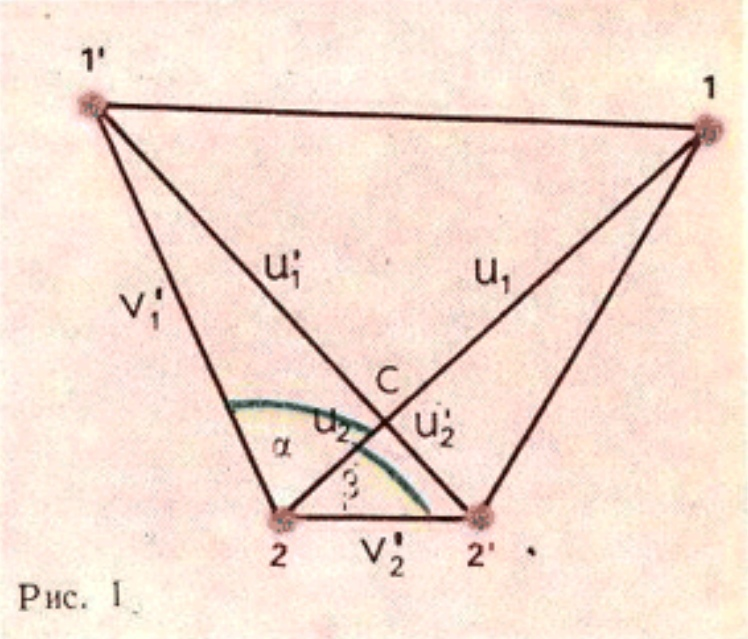
\includegraphics[scale=0.3]{ris_1.jpg}\par
\textbf{2.} Из диаграммы рассеяния частиц с одинаковыми массами (рис. 6 на стр. 23) найдем, что угол отдачи равен $30^\circ$, скорость $\alpha$-частицы после рассеяния $v_\alpha'=v_\alpha\cos60^\circ=\frac{1}{2}v_\alpha$, а скорость ядра отдачи $v_\textmd{\footnotesize я}=v_\alpha\cos30^\circ=\frac{\sqrt{3}}{2}v_\alpha$ ($v_\alpha$ - скорость $\alpha$-частицы до столкновения с ядром). Поэтому энергия $\alpha$-частицы после рассеяния
\end{multicols}
\newpage
\setcounter{page}{32}
В качестве примера приведем таблицы умножения и сложения в 7-арифметике.\newline\newline
\begin{minipage}{0.4\textwidth}
$$\textbf{Таблица умножения}$$
\begin{center}
\begin{tabular}{c|c c c c c c}
  $\times$ & 1 & 2 & 3 & 4 & 5 & 6\\ \hline
  1 & 1 & 2 & 3 & 4 & 5 & 6\\
  2 & 2 & 4 & 6 & 1 & 3 & 5\\
  3 & 3 & 6 & 2 & 5 & 1 & 4\\
  4 & 4 & 1 & 5 & 2 & 6 & 3\\
  5 & 5 & 3 & 1 & 6 & 4 & 2\\
  6 & 6 & 5 & 4 & 3 & 2 & 1\\
\end{tabular}
\end{center}
\end{minipage}
\begin{minipage}{0.4\textwidth}
$$\textbf{Таблица сложения}$$
\begin{center}
\begin{tabular}{c|c c c c c c c}
  + & 0 & 1 & 2 & 3 & 4 & 5 & 6\\
  \hline
  0 & 0 & 1 & 2 & 3 & 4 & 5 & 6\\
  1 & 1 & 2 & 3 & 4 & 5 & 6 & 0\\
  2 & 2 & 3 & 4 & 5 & 6 & 0 & 1\\
  3 & 3 & 4 & 5 & 6 & 0 & 1 & 2\\
  4 & 4 & 5 & 6 & 0 & 1 & 2 & 3\\
  5 & 5 & 6 & 0 & 1 & 2 & 3 & 4\\
  6 & 6 & 0 & 1 & 2 & 3 & 4 & 5\\
\end{tabular}
\end{center}
\end{minipage}